\chapter{The NOvA experiment}\label{sec:NOvA}
%%% OVERVIEW OF THE NOvA EXPERIMENT %%%

The NuMI Off-axis $\nu_e$ Appearance (NOvA) experiment \cite{NOvAWebsite} is a long-baseline neutrino oscillation experiment based at the Fermi National Accelerator Laboratory (Fermilab) \cite{FNALWebsite}. NOvA receives an off-axis $\nu_\mu$ and $\overline{\nu}_\mu$ beam from Fermilab's NuMI neutrino source, described in Sec.~\ref{fig:NOvANuMI}, and measures $\nu_e$/$\overline{\nu}_e$ appearance and $\nu_\mu$/$\overline{\nu}_\mu$ disappearance between its two highly active and finely segmented detectors, described in Sec.~\ref{fig:NOvADetectors} \cite{PhysicsOfNOvA.pdf}. 

The capability to measure both $\nu_e$ and $\overline{\nu}_e$ appearance, coupled with a significant matter effect induced by the long baseline, allows NOvA to address some of the most important questions in neutrino physics to date, such as the neutrino mass ordering, the octant of $\theta_{23}$, and the possible CP violation in the neutrino sector \cite{PhysicsOfNOvA.pdf,NOvAStatusAndOutlook.pdf,FirstNOvAResult.pdf,2019NOvAFHCRHCResults.pdf,NOvAResults2021.pdf}. NOvA also measures the values of $\theta_{13}$, $\theta_{23}$ and $\left|\Delta m^2_{atm}\right|$ \cite{PhysicsOfNOvA.pdf}, but also measures neutrino differential cross sections in the near detector \cite{NOvANCPi0XSecMeasurement2019.pdf, NOvANumuCCXSexMeasurement2023.pdf, NOvANueCCXSecMeasurement2023.pdf, NOvANuMuCCPi0XSecMeasurement2023.pdf}, provides constraint on the possible sterile neutrino models \cite{NOvASterilesFHCResults2017.pdf, NOvASterilesFHCRHCResults2021.pdf}, monitors for supernova neutrino activity \cite{NOvASupernovaMeasurements2020.pdf, NOvASupernovaCoincidenceMeasurements2021.pdf}, searches for magnetic monopoles \cite{NOvASlowMagMonopoles2021.pdf}, or constrains neutrino electromagnetic properties (this thesis) amongst other topics. Using two functionally identical detectors mitigates the systematic uncertainties of neutrino oscillation measurements, described in Sec.~\ref{sec:NOvASystematics}.

\note{Should I mention here when did NOvA start taking data and how long is it planning to run for? Maybe future analysis? Size of the collaboration? - YES!}

\section{The Neutrino Beam}\label{sec:NuMI}

The neutrino beam for NOvA comes from the Fermilab-based \textit{Neutrinos at the Main Injector} (NuMI) neutrino source \cite{NuMI.pdf}. The schematic description of NuMI is shown on Fig.~\ref{fig:NOvANuMI}, starting on the left hand side with $\unit[120]{GeV}$ protons from the Main Injector, part of the Fermilab accelerator complex. The proton beam is divided into $\unit[10]{\mu s}$ long pulses, with $\sim5\times 10^{13}$ protons on target (POT) per spill every $\sim\unit[1.3]{s}$ long cycle time, resulting in a proton beam power of $\sim\unit[800]{kW}$, with upgrades currently underway to surpass $\unit[1]{MW}$ \cite{NuMIUpgradeToMWProceedings2022.pdf}.

\begin{figure}[!hbtp]
\centering
%is pdf-a
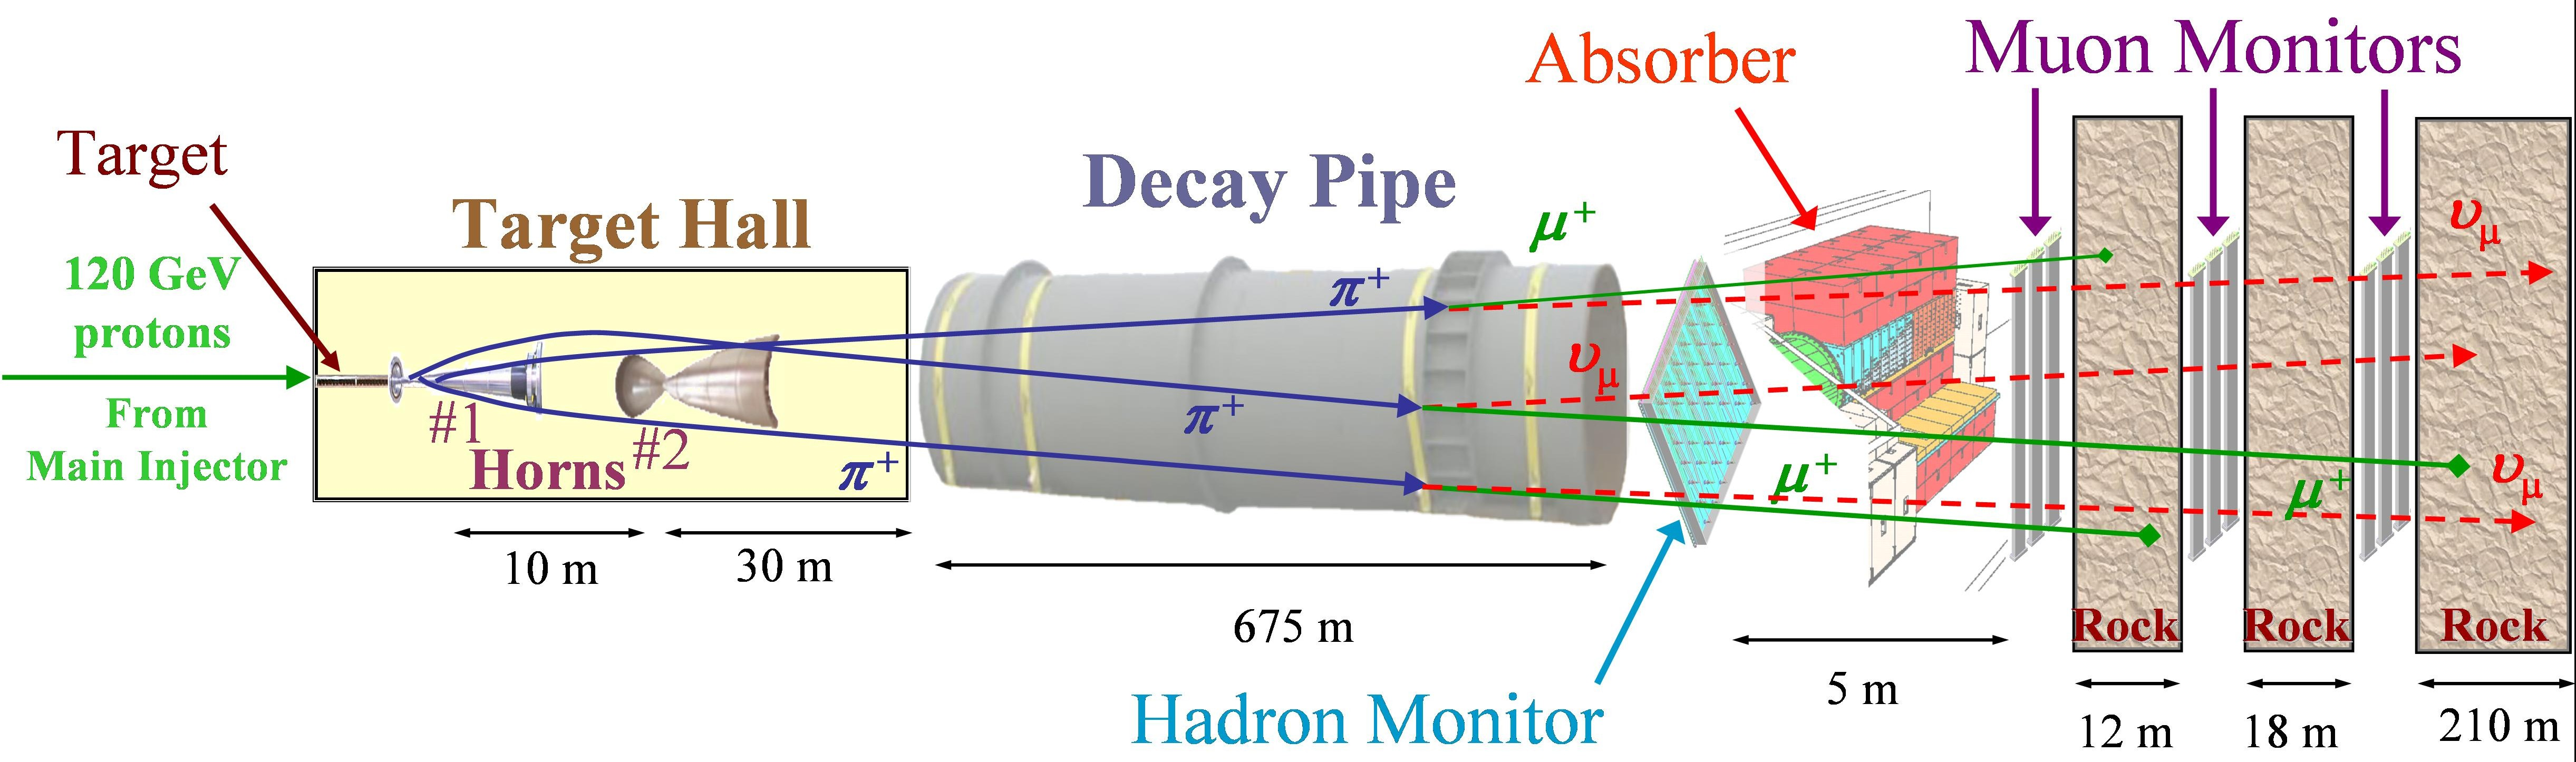
\includegraphics[width=\textwidth]{Plots/NOvAExperiment/BeamlineAlternative.jpg}
\caption[The schematic of the NuMI beam facility]{
The NuMI neutrino beam starts on the left hand side with protons from the Main Injector impinged on a graphite target producing mainly pions and kaons. These are then focused and charge-selected by two focusing horns, after which they decay inside the decay pipe into a high-purity muon neutrino, or antineutrino beam. The residual hadrons are stopped and monitored in the hadron absorber and the remaining muons are recorded with muon monitors and absorbed inside the rock.
%The schematic of the NuMI beam facility. The beam travels from left to right. The individual components shown are not to scale. Protons originate as $H^-$ ions, which are converted into protons in the Booster, sent to the main injector, where they are finally accelerated to $120\,\si{\giga\electronvolt}$, bent downward by $58\,\si{\milli\radian}$ and transported $350\,\si{\meter}$ to the $1.2\,\si{\meter}$ long NuMI target. The protons are incident on the graphite target and the produced hadrons are focused by two magnetic horns, located in about $40\,\si{\meter}$ long target hall, with about $19\,\si{\meter}$ separation between the two horns. Hadrons then enter a $675\,\si{\meter}$ long decay pipe made of steel, with $2\,\si{\meter}$ diameter, which serves as vacuum or low density environment for the mesons to propagate and decay into tertiary mesons, charged leptons and neutrinos. A hadron monitor is located at the end of the decay volume just in front of the $5\,\si{\meter}$ thick aluminium, steel and concrete absorber to record the profile of the residual hadrons. Of the particles interacting in the absorber, the principal component (approximately $80\%$) is the proton beam that has not interacted. The remainder are mainly mesons which have not decayed in the pipe or secondary protons. The absorber not only stops most of the particles still remaining in the beam but also acts as a shield against radiation. Muons and neutrinos deposit little or no energy in the absorber and continue into unexcavated rock with three muon monitors allowing measurement of the residual muon flux. The $240\,\si{\meter}$ of rock following the absorber stops the muons remaining in the beam but allows the neutrinos to pass\cite{numi}. 
}
\label{fig:NOvANuMI}
\end{figure}

The proton beam passes through a collimating baffle before hitting a $\sim\unit[1.2]{m}$-long graphite target \cite{LEOFluxPredictionAtNuMI.pdf}, producing hadrons, predominantly pions and kaons \cite{NuMI.pdf}. These are then focused and selected by two parabolic magnetic "horns". Using a positive current inside the horns focuses positively charged particles, which then decay into neutrinos, and removes negatively charged particles. Reversing the horn current on the other hand focuses negatively charged particles, which decay into antineutrinos, and defocuses positively charged particles. The neutrino mode is therefore called Forward Horn Current (FHC) and the antineutrino mode is called Reverse Horn Current (RHC). The composition of the neutrino beam for both these modes at the NOvA near detector, shown as a rate of charge current events, is presented on Fig.~\ref{fig:NOvABeamComponents}, displaying the very high purity of $\nu_\mu$ component in the FHC beam, and the high purity of $\overline{\nu}_\mu$ component in the RHC mode \cite{NuMI.pdf}.

\begin{figure}[!htb]  
  \centering
  \includegraphics*[width=.495\textwidth]{Plots/NOvAExperiment/NuMIBeamComponentsCCEvtsFHC.pdf}
  \noindent\centering
  \includegraphics*[width=.495\textwidth]{Plots/NOvAExperiment/NuMIBeamComponentsCCEvtsRHC.pdf}
  \caption[NuMI neutrino beam components in the NOvA near detector]{The charge current event rates for different neutrino flavours, as measured at the NOvA Near Detector in the FHC regime shown on the left, or the RHC regime on the right. The contribution of neutrino flavours to the event rates is also displayed, showing the high purity of the neutrino beam for NOvA.}
 \label{fig:NOvABeamComponents}
\end{figure}

The focused hadrons pass through a $\unit[675]{m}$-long decay pipe filled with helium to create a low density environment for hadrons to propagate and decay into neutrinos, or antineutrinos \cite{NuMI.pdf,LEOFluxPredictionAtNuMI.pdf}. High energy hadrons that do not decay in the decay pipe are absorbed within a massive aluminium, steel and concrete hadron absorber and monitored with a hadron monitor \cite{NuMI.pdf}. The leftover muons are ranged out in a dolomite rock after the absorber and monitored using three muon monitors. The hadron and all the muon monitors are ionization chambers, used to monitor the quality, location and relative intensity of the beam \cite{NuMI.pdf}.

The resulting neutrino beam is peaked $\sim\unit[7]{GeV}$ with a wide energy band. However, thanks to the kinematics of the dominant pion decay, by placing NOvA detector $\unit[14.6]{mrad}$ ($\approx\unit[0.8]{\degree}$) off the main NuMI beam axis, we achieve a narrow band neutrino flux peaked at $\unit[1.8]{GeV}$ \cite{NOvAResults2021.pdf,NOvATechreport.pdf}, as can be seen on Fig.~\ref{fig:NOvAOffAxis}. Using an off-axis neutrino flux increases the neutrino beam around $\unit[2]{GeV}$ about 5-fold compared to the on-axis flux and enhances background rejection for the $\nu_e$ appearance analysis \cite{NOvATechreport.pdf}.

%Protons originate as $\textsc{H}^-$ ions, accelerated by the Linac to $\unit[400]{MeV}$, converted to protons and further accelerated to $\unit[8]{GeV}$ in the Booster, to be passed to the Main Injector which finally accelerates them to $\unit[120]{GeV}$ . Protons are then extracted, bent down to point towards the MINOS/NOvA Far Detector, and transported to the NuMI target \cite{NuMI.pdf}. The current beam power is $\sim\unit[700]{kW}$ with a plan \cite{PIP2.pdf} of reaching more than $\unit[1]{MW}$ beam power in the future upgrades.
%The NuMI target is a graphite fin, $\unit[7.4]{mm}$ wide, $\unit[63]{mm}$ tall and $\approx\unit[120]{cm}$ long (along the beam direction)\footnote{Previous target proportion were $\unit[6.4]{mm}$ W, $\unit[15]{mm}$ H and $\unit[95.38]{cm}$ L used in low energy design (see lower) \cite{NuMI.pdf}.} \cite{LEOFluxPredictionAtNuMI.pdf}. Protons interact in the target producing hadrons, predominantly pions and kaons \cite{NuMI.pdf}.

%The off-axis location means that both NOvA detectors are sited $14.6\,\si{\milli\radian}$ off the NuMI beam axis, in contrast to the MINOS Far Detector. This is because at around $14\,\si{\milli\radian}$, the energy of the neutrino does not have a strong dependence on the energy of the parent pion (fig. \ref{angleoff}), and also at this angle, the medium energy beam produces a narrow energy beam with approximately five times more neutrinos at $2\,\si{\giga\electronvolt}$ (fig. \ref{off-axis}), which is well-matched to the oscillation maximum expected to be at $1.6\,\si{\giga\electronvolt}$, thus maximizing the experiment’s neutrino oscillation sensitivity. In addition to the increased flux, the narrowness of the off-axis spectra enhances background rejection.\cite{techreport}

\begin{figure}[!htb]  
  \centering
  \includegraphics*[width=.48\textwidth]{Plots/NOvAExperiment/PionOffAxis.pdf}
  \noindent\centering
  \includegraphics*[width=.51\textwidth]{Plots/NOvAExperiment/OffAxisFluxPionEmbedded.pdf}
  \caption[The NOvA off-axis beam concept]{Dependence of the neutrino energy on the parent pion's energy and a neutrino energy distribution for an on-axis beam and three different off-axis beam designs. The case for NOvA is shown here in red and results in a narrow neutrino energy distribution around $\unit[2]{GeV}$, independent on the parent pion's energy.}
 \label{fig:NOvAOffAxis}
\end{figure}

\section{The NOvA Detectors}\label{sec:NOvADetectors}

The two main NOvA detectors are the Near Detector (ND), located in Fermilab $\sim\unit[1]{km}$ from the NuMI target and $\sim\unit[100]{m}$ under ground, and the Far Detector (FD), located $\sim\unit[810]{km}$ from Fermilab at Ash River in north Minnesota, partially underground with a rock overburden \cite{NOvATechreport.pdf}. NOvA also operated a detector prototype called Near Detector on the Surface (NDOS) used for an early research and development of detector components and analysis \cite{NOvAStatusAndOutlook.pdf}. Additionally, NOvA operated a NOvA Test Beam detector (TB), described in detail in Sec.~\ref{sec:TBDetector}. The scale of the near and far detectors are shown on Fig.~\ref{fig:NOvADetectors}.

\begin{figure}[ht]
\centering
%is pdf-a
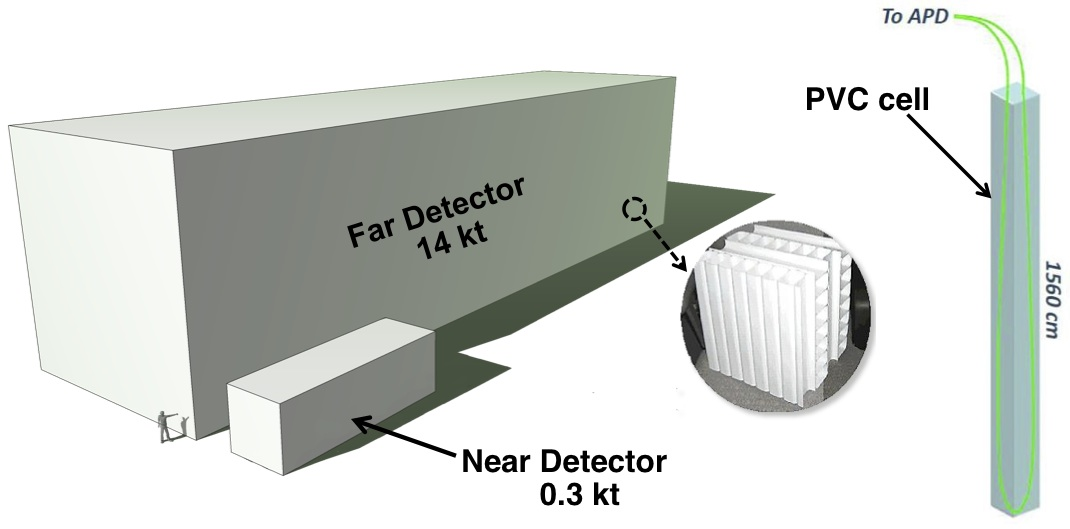
\includegraphics[width=1\textwidth]{Plots/NOvAExperiment/NOvADetectors.png}
\caption[NOvA detectors]{Schematic description of scale and composition of the NOvA detectors. Inset showing the orthogonal planes of PVC cells. One cell containing liquid scintillator and a loop of wavelength sifting fibre attached to an avalanche photodiode is also shown \cite{NeutrinoDetectorsForOscExp.pdf}. The length of the cell corresponds to a far detector cell.}
\label{fig:NOvADetectors}
\end{figure}

All NOvA detectors are highly segmented, highly active, functionally identical tracking calorimeters made up of polyvinyl chloride (PVC) cells filled with liquid scintillator. Each cell is a hollow cuboid with cross section of $\unit[5.6]{cm}\times\unit[3.6]{cm}$ (with some variations) and extending to the full width/height of each detector, which is $\approx\unit[4]{m}$ for the ND and $\approx\unit[15]{m}$ for the FD \cite{NOvATechreport.pdf}. An example of a FD cell is shown on the right of Fig.~\ref{fig:NOvADetectors}.

Cells are connected side-by-side in a 16 cell-wide extrusions with $\unit[3.7]{mm}$-wide walls between cells and $\unit[5.1]{mm}$-wide walls on the outsides of the extrusions. The first and last cell of each extrusion are $\sim\unit[3]{mm}$ narrower than the rest of the cells\footnote{All of the values for detector, planes and cells size and number were adjusted to the most recent detector specification from an internal NOvA documentation.}. Two extrusions are connected side-by-side to form a 32 cell-wide \textit{module}, with each module having a separate readout. In the FD, 12 modules are connected side-by-side to form a \textit{plane}, whereas in the ND only 3 modules make up a plane. Planes are positioned one after another, alternating between vertical and horizontal orientation, and grouped into diblocks, each containing 64 planes. The FD contains 14 diblocks, totalling 896 planes, whereas the ND contains 3 diblocks totalling 192 planes. However, the ND also consists of a Muon Catcher region, positioned right after the active region, consisting of 22 planes of the normal NOvA detector design, 2 modules high and 3 modules wide, sandwiched with 10 steel plates to help range out muons from $\nu_\mu$ charge current interactions \cite{NOvAStatusAndOutlook.pdf,NOvATechreport.pdf}.

Each cell is filled with a liquid scintillator, with a single wavelength shifting fibre $2\times$ the length of the cell, looped at the end. The liquid scintillator consists of mineral oil with $4.1\%$ pseudocumene as the scintillant, producing light with wavelength between $\unit[360-390]{nm}$, and additives to shift the initial light to $\unit[400-450]{nm}$ to match the absorption spectrum of the fibres.

%%%%%%%%%%%%%%%%%%%%%%%%%%%%%%%%%%%%%%%%%%%%%%%%%%%%%%%%%%%%%%%%%%%%%%%%%%%%%%%
%%% Master's thesis on NOvA detectors:
\iffalse
The liquid scintillator amounts for about $63\%$ of the total detector mass (the rest being the PVC structure) \cite{NeutrinoDetectorsForOscExp.pdf} and consists primarily of mineral oil with $4.1\%$ pseudocumene [1,2,4-Trimethybenzene] as the scintillant \cite{NOvATechreport.pdf}. The radiation length in the detector ($\unit[38]{cm}$) is many times larger than the cell dimensions, which allows for a good reconstruction and separation of electromagnetic and hadronic showers, identification of muons and neutral pions \cite{NOvAStatusAndOutlook.pdf}.

Charged particles in the detector produce a scintillator light captured by the wavelength-shifting fibre directing it to one pixel on an APD mounted at the top of each cell. APD converts the light into electrical signal, which is then amplified, digitized and consolidated by the Data Concentrate Module into $\unit[5]{ms}$ time slices, buffered for a minimum of $\unit[20]{s}$ waiting for a spill trigger and finally written to a file for storage or shared memory for monitoring \cite{NOvADAQ.pdf}.

We are using the minimum ionizing part of cosmic-ray muon tracks that stop in the detectors to calibrate the absolute energy scale to within $\pm 5\%$ \cite{2019NOvAFHCRHCResults.pdf}. GEANT4 \cite{GEANT4.pdf} simulation is used to calibrate the deposited energy of individual particles as well as the scintillation light, light transport and readout response \cite{NOvASimulationOld-Fluka.pdf}.

Since most of the primary goals of NOvA depend on successfully observing $\nu_e$ charged-current interaction, the reconstruction chain was tailored for this task \cite{NOvAReco.pdf}. Different interactions as seen in a NOvA detector are shown on fig.\ref{interactions}. Reconstruction begins by clustering hits into slices by time and space "density". Than a modified Hough transform identifies prominent features, which are used to determine the global 3D vertex for the slice. This vertex is used in the fuzzy k-means algorithm to produce prongs (a collection of cell hits with a start point and a direction) which are fed to a neural network to classify the degree to which the slice was like a $\nu_e$ CC (or other) interaction \cite{NOvAReco.pdf}. NOvA uses a convolutional neural network called Convolution Visual Network (CVN) originally based on the GoogLeNet architecture. CVN identifies neutrino interactions based on their topology and therefore without the need for detailed reconstruction \cite{CVN.pdf}.

\begin{figure}[ht]
\centering
%is pdf-a
\includegraphics[width=1\textwidth]{/home/robo/Documents/S-cool/DIPLO/img/nova/eventtopology_embedded-page-001.jpg}
\caption[NOvA detectors event topologies]{Different event topologies as seen in NOvAs detectors with corresponding feynman diagrams. Figure is from \cite{NOvAInteractionsPlot.pdf}.}
\label{interactions}
\end{figure}
\fi
%%%% End of master's thesis for detectors
%%%%%%%%%%%%%%%%%%%%%%%%%%%%%%%%%%%%%%%%%%%%%%%%%%%%%%%%%%%%%%%%%%%%%%%%%%%%%%%

\todo{List the percent-wise contribution of elements in the NOvA soup.}

\note{The MIP energy loss for electrons (similarly to muons) can be found with a similar method as used in the AbsCal\_technote\_1stAna in TestBeam (page 2).}

\section{Data Acquisition}\label{sec:DAQ}

APDs and how they work are pretty well described in the NOvA technical design report. For some reason the TDR I have downloaded doesn't have the full chapter 14. Full TDR can be found in docdb:2678 chapter by chapter.

APD signal first needs to be converted to a digital format with ADC (is there anything before that?). Maybe take a look at docdb:353.

This digital signal is then passed to the FPGA, which does the correlated sampling and time stamping [docdb:353].
\note{From docdb:353}

\begin{figure}[!htb]  
  \centering
  \includegraphics*[width=.495\textwidth]{Plots/NOvAExperiment/NOvAAPDMountedWithLabels.jpg}
  \noindent\centering
  \includegraphics*[width=.495\textwidth]{Plots/NOvAExperiment/NOvAAPDBottomWithLabels.jpg}
  \caption[NOvA Avalanche Photo Diods]{The Avalanche Photo Diods for NOvA}
 \label{fig:NOvAAPD}
\end{figure}

\begin{figure}[!htb]  
  \centering
  \includegraphics*[width=\textwidth]{Plots/NOvAExperiment/NOvAFEBWithLabels.jpg}
  \caption[NOvA Front End Board]{The Front End Board for NOvA}
 \label{fig:NOvAFEB}
\end{figure}

TDR:
Major components are the carrier board connector location at the left, which brings the APD signals to the NOvA ASIC, which performs integration, shaping, and multiplexing. The chip immediately to the right is the ADC to digitize the signals, and FPGA for control, signal processing, and communication.
The front end electronics has the responsibility of amplifying and integrating the signals from the APD arrays, determining the amplitude of the signals and their arrival time and presenting that information to the data acquisition system (DAQ).
Data from the ADC is sent to an FPGA where multiple correlated sampling is used to remove low frequency noise. This type of Digital Signal Processing (DSP) also reduces the noise level and increases the time resolution.

We are saving all the ADC and TDC (Time Digital Converter I believe) values to the RawDigit. Then they are fitting in the Calibrator to a functional form and converted to PE by fitting for the peak ADC.

"The chip will be used in its “Analog” mode in NOvA. In this mode, eight channels of integrator/shaper outputs are fed onto a multiplexer and driven by a differential amplifier onto the output pads. The multiplexer runs at 16 MHz, sending its signal output to the quad ADC. The ADC outputs, in turn, are sent in a continuous stream to an FPGA which processes the data and outputs it onto a data link. In these tests, the data link is standard USB 2.0" [docdb:1904]

DAQ Software (what happens to the signal after the FEBs) is described in docdb:1233. Not sure if this is the final design though. 

Triggers

%The NOvA calibration process technically also involves \textbf{timing calibration}, which corrects for the time differences of the signal to be processed \cite{NinerThesis}. However, this is done as a separate project to the relative and absolute calibrations and is out of scope of this technical note.

\section{Data Processing and Event Reconstruction}
Basic description of the process from raw data to final predictions (or just cafs?)

Maybe talk about data quality as well? Good runs and so on...

Reconstruction - describe the reconstruction tools used to get the final products, focusing on the electron reconstruction.

Clustering into slices - how is that done?

Reconstruction of prongs and tracks. Electron showers

\section{Simulation}\label{sec:NOvASimulation}

\subsection{Neutrino Beam Simulation}
Should I mention that in the past we used Fluka, but now we're using Geant4

%%%%%%%%%%%%%%%%%%%%%%%%%%%%%%%%%%%%%%%%%%%%%%%%%%%%%%%%%%%%%%%%%%%%%%%%%%%%%%%
%%%% Master's thesis on flux simulation
\iffalse
NOvA uses GEANT4-based \cite{GEANT4.pdf} Monte Carlo (MC) simulation called g4numi \cite{LEOFluxPredictionAtNuMI.pdf} to calculate the production and transportation of the neutrino flux through the beamline components and ends when a neutrino is created. From there GENIE event generator \cite{GENIE.pdf} simulates neutrino interactions in the detector \cite{2019NOvAFHCRHCResults.pdf} and another GEANT4 simulates the detector response \cite{NOvASimulationOld-Fluka.pdf}. 

The simulation starts with a $\unit[120]{GeV}$ kinetic energy primary proton beam entering the NuMI target \cite{NuMIFlux.pdf}. There are often multiple interactions within the target and in the materials downstream of it and since the hadron production process is governed by non-perturbative QCD and occurs in the nucleus, highly accurate theoretical predictions are not possible \cite{NuMIFlux.pdf,LEOFluxPredictionAtNuMI.pdf}. NOvA therefore tunes and corrects possible mismodeling of the model using external data in a package developed for MINERvA experiment called Package to Predict the Flux (PPFX) \cite{LEOFluxPredictionAtNuMI.pdf}. NOvA also tunes the cross-section model of the GENIE simulation to the ND data to reduce uncertainties in the extrapolation of measurements on the ND to the FD \cite{2019NOvAFHCRHCResults.pdf}.


%In principle, precise knowledge of π and K production cross sections on the target material, and of the focusing properties of the beamline, should translate into a well known neutrino flux. In practice the situation is more complicated, since there are often multiple interactions within the target, and in the materials downstream of it. Also, the meson production process is governed by nonperturbative QCD and occurs in a nucleus, so highly accurate, first principle, theoretical predictions are not available. Neutrino experiments have usually dealt with this situation by producing detailed simulations of the beamline materials and geometry coupled with phenomenological models of hadronic cascades, such as those in Geant4 [1] and FLUKA [2, 3]. Those models are not necessarily accurate but can be tuned or benchmarked by comparing their predictions to measurements of hadron production. Recent measurements of pion production on a thick (two interaction length) carbon target have been released by MIPP [4], and measurements of pion production on a thin (few per cent interaction length) carbon target are available from NA49 [5]. In addition, there are several other hadron production measurements on various materials, using both proton and pion beams, that can be used to constrain a neutrino beamline simulation.[NuMIFlux.pdf]

%The simulation accounts for all particle interactions and propagation in the beamline, starting with protons entering the carbon target and ending in decays that produce a neutrino. The simulation outputs the location and kinematic information of each decay producing a neutrino. The neutrino flux at a particular location is then determined by using the differential decay rate, as a function of solid angle, given the neutrino species and the parent particle’s kinematic information. Roughly 85% of the interactions that produce particles that lead to muon neutrinos passing through MINERvA are from protons interacting on carbon. Other relevant materials are aluminum (horns), iron (decay pipe walls), helium (decay pipe gas), and air (target hall). Interactions of π ± , K ± and n created in the initial proton interaction, or subsequent interactions, are subdominant but non-negligible. Table I summarizes the hadronic interactions that lead to ν μ that pass through MINERvA. When protons collide with carbon, the interactions can produce pions, kaons, neutrons, strange baryons, and lower energy protons. These particles, if they do not decay first, can interact either in the target or in other downstream material to create tertiary particles that can also decay into neutrinos. \cite{NuMIFlux.pdf}
\fi
%%% End of master's on flux simulation
%%%%%%%%%%%%%%%%%%%%%%%%%%%%%%%%%%%%%%%%%%%%%%%%%%%%%%%%%%%%%%%%%%%%%%%%%%%%%%%


\subsubsection{Package to Predict the FluX}
Should I talk about this now or should I talk about the simulations (and their corrections) together? 
%Good description of PPFX, beam transport and the principal components is in the NOvA-T2K technote for Flux (doc-db:54582) https://nova-docdb.fnal.gov/cgi-bin/sso/ShowDocument?docid=54582

I did this in the beginning of my thesis so maybe I should mention this. Especially the possible improvements and what I've done for them (enough to say I looked at it?)

%%%%%%%%%%%%%%%%%%%%%%%%%%%%%%%%%%%%%%%%%%%%%%%%%%%%%%%%%%%%%%%%%%%%%%%%%%%%%%%
%%% PPFX from master's thesis

\iffalse
PPFX is used to correct each interaction of neutrino's ancestry chain by weighting it with a factor computed from external experimental measurements of yields or invariant differential cross-sections: \cite{LEOFluxPredictionAtNuMI.pdf}
\begin{equation}
c_{i}=\frac{N^{data}_{i}}{N^{MC}_{i}},
\end{equation}
where $i$ denotes either initial or final state.

This weighting factor depends on the identity of prejectile, target, hadrons and also on the initial and final state kinematics \cite{LEOFluxPredictionAtNuMI.pdf}. The kinematical distributions of the most dominant hadrons, pions and kaons, after leaving the target, are shown on fig.\ref{PionKaonPtPzSpace}. 

The kinematical values of the initial particles (like the initial $\unit[120]{GeV}$ proton interacting on carbon in NuMI) are not always the same between the measured interaction and the required values. To solve this we use the \textit{Feynman-x} ($x_{F}$) scaling variable, which is defined as:
\begin{equation}
x_{F}\equiv\frac{p_{\parallel}^{*}}{p_{\parallel}^{*}\left(max\right)}\simeq\frac{2p_{\parallel}^{*}}{\sqrt{s}},
\end{equation}
where $p_{\parallel}^{*}$ is the longitudinal momentum in the center of mass (CMS) frame and it's maximum value $p_{\parallel}^{*}\left(max\right)\simeq\sqrt{s}/2$ ($\sqrt{s}$ is the energy of the CMS). Feynman speculated \cite{feynman1969.pdf} that expressing the cross-sections of inclusive high energy hadronic collisions in terms of $x_{F}$ would make the cross-section scaling energy independent  \cite{LEOFluxPredictionAtNuMI.pdf}.
%$c_i$ is the \textit{central value} of the weight

PPFX makes two corrections:
\begin{itemize}
\item Attenutation correction,
\item Particle production correction.
\end{itemize}

Attenuation correction is for the probability that a particle interacts (or not) within a material while crossing a distance $r$, while the particle production correction is for the instances when an interaction does happen. This corrections depend on the agreement between the predicted and measured cross-section \cite{LEOFluxPredictionAtNuMI.pdf}.

There are two main experiments whose results are used in the PPFX. NA49 \cite{NA49:Inclusive_production_of_charged_pions.pdf}, which used $\unit[158]{GeV}$ protons interacting on carbon thin target, and MIPP \cite{pionToKaonIn_pC.pdf} which used protons from the Main Injector and both thin carbon target and the low energy NuMI target (thick target) \cite{PPFXTechnote2017.pdf}. Energy scaling of the external data to calculate the PPFX weight is performed by FLUKA and for example for the NA49 data looks like \cite{NuMIFlux.pdf}

%%% Hadron production datasets:
%There are two major datasets available to constrain the process where protons interact on carbon and produce charged pions. One measurement, from NA49 [5], uses a thin target with an incident proton momentum of 158 GeV/c. The other measurement, from MIPP [4], uses an actual NuMI LE target and 120 GeV/c protons. These two datasets will be used to make separate “thin target” and “thick target” flux predictions by weighting each interaction leading to a neutrino going through MINERvA. We also use additional datasets to constrain kaon and nucleon production, and the absorption of particles in beamline materials. Where multiple interactions are constrained with data, the overall weight applied to the neutrino event is simply the product of the weights for each interaction.\cite{NuMIFlux.pdf}

\begin{equation}
c\left(x_{F},p_{T},p\right)=\frac{f_{Data}\left(x_{F},p_{T},p_{0}=\unit[158]{GeV/c}\right)}{f_{MC}\left(x_{F},p_{T},p_{0}=\unit[158]{GeV/c}\right)}\times scale\left(x_{F},p_{T},p\right),
\end{equation}
where
\begin{equation}
scale\left(x_{F},p_{T},p\right)=\frac{\sigma_{FLUKA}\left(x_{F},p_{T},p\right)}{\sigma_{FLUKA}\left(x_{F},p_{T},p_{0}=\unit[158]{GeV/c}\right)}.
\end{equation}

For kaons with $x_{F}<0.2$ PPFX uses weights based on NA49 measurements\cite{NA49DataKaons.pdf} and for kaons with $0.2<x_{F}<0.5$ PPFX uses the $K/\pi$ yield ratio from the MIPP thin target measurements\cite{pionToKaonIn_pC.pdf} multiplied by NA49 thin target yields. $p_{T}-p_{z}$ distribution of the PPFX weights for pions and kaons are shown on fig.\ref{PPFXWgtsPionKaonFig}.
\fi

%%% End of master's thesis on PPFX
%%%%%%%%%%%%%%%%%%%%%%%%%%%%%%%%%%%%%%%%%%%%%%%%%%%%%%%%%%%%%%%%%%%%%%%%%%%%%%%

\subsubsection{Constraining the Hadron Production Systematic Uncertainty in NOvA}
Again, should I discuss it here or somewhere else? Maybe not necessary as a full section. Not sure if I should include a discussion on nu-on-e, or low nu studies here, or just PPFX improvements.

\subsection{Simulation of the Neutrino Interactions}

\subsubsection{NOvA Reweight of the Neutrino Interaction Predictions}

\subsection{Simulation of the Detector Response}
Should I join this with the other simulation subsection?

%%%%%%%%%%%%%%%%%%%%%%%%%%%%%%%%%%%%%%%%%%%%%%%%%%%%%%%%%%%%%%%%%%%%%%%%%%%%%%%
%%%%%%%%%                   Detector calibration                     %%%%%%%%%%
%%%%%%%%%%%%%%%%%%%%%%%%%%%%%%%%%%%%%%%%%%%%%%%%%%%%%%%%%%%%%%%%%%%%%%%%%%%%%%%
\section{Detector Calibration}\label{sec:NOvACalibration}
%%% General introduction to calibration
The purpose of calibration is to make sure that we get the same amount of energy wherever or whenever it's deposited in whichever of NOvA's detectors and to express this amount of energy in physical units. The NOvA calibration uses cosmic ray muons, which provide a consistent, abundant, and well-understood source of energy deposition.

%. The main aims are to correct for the attenuation of light along fibers, to remove differences in energy deposition within the detector, and to provide an absolute energy scale from collected charge to physical energy units. [TB paper]

%%% Calibration samples, trigger, reconstruction, and selection. Also simulation, fiber brightness and so on...

\subsubsection*{Creating calibration samples}\label{secCreatingCalibrationSamples}

We want to select good quality cosmic ray muons. First, we remove beam related events based on their time stamps relative to the time of the beam spill. Next we apply reconstruction to get the CellHit, slicer, and track information, followed by a track-based selection to remove misreconstructed and poor quality events.

Since energy deposition depends on the path length particle travels through a cell, we only use hits for which we can reliably calculate their path length. We call these hits \textbf{tricell} hits, as we require that all accepted hits are accompanied by a recorded hit in both neighbouring cells of the same plane, as shown on Fig. \ref{figTricellCondition}. In case there is a bad channel in a neighbouring cell, we ignore this channel and look one cell further. We can then calculate the path length simply as the cell width divided by the cosine of the direction angle \cite{NOVA-doc-13579,NOVA-doc-7410}.

\begin{figure}[hbtp]
\centering
\begin{subfigure}[b]{0.49\textwidth}
\centering
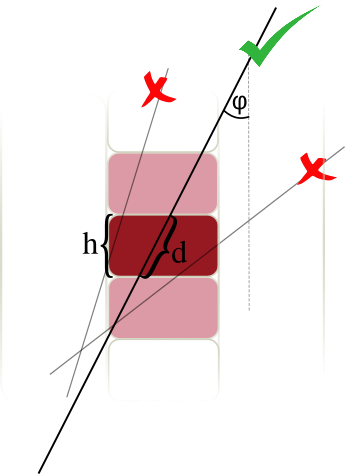
\includegraphics[width=0.6\textwidth]{Plots/NOvAExperiment/TricellConditionWithDescription.png}
\caption{}
\end{subfigure}
\begin{subfigure}[b]{0.49\textwidth}
\centering
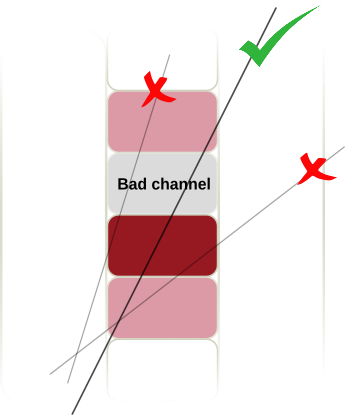
\includegraphics[width=0.6\textwidth]{Plots/NOvAExperiment/TricellConditionWithBadChannel.png}
\caption{}
\end{subfigure}
\caption{Illustration of the tricell condition (a). We only use hits that have two surrounding hits in the same plane to be used in the NOvA calibration. This is to ensure a good quality of the path length (d) reconstruction, which is calculated from the known cell height (h) and the reconstructed track angle $\left(\varphi\right)$. In case the hit is next to a bad channel (b), we ignore this bad channel and require a hit in the next cell over.}
\label{figTricellCondition}
\end{figure}

%The first step in the attenuation calibration is to select the suitable hits from tracks of cosmic ray muons. Because a reliable estimate of pathlength is required, not all hits are suitable for use.  If a cell has each of its neighbors in the same plane hit, then we know, for a Y view cell, that the track entered through the upper wall, and exited through the lower wall. The pathlength then is just the width of the cell divided by the direction cosine. This selection also significantly decreases the chance that the hit in question is a noise hit. Allowance is made for neighboring dead cells, so e.g. “hit, dead, hit, hit” would still lead the 3rd cell to be selected. The second best hit selection, in cases where there are too many dead neighboring cells on each side, is the so-called “z” estimator, where a hit is required at the same cell number in each of the neighboring planes in the same view. The pathlength is then the ratio of cell depth to cz.[docdb:13579 - SA The Attenuation and Threshold Calibration of the NOvA detector, copied from docdb:7410]

%from docdb:7410: A requirement that the track be “throughgoing” (lowest endpoint outside the fiducial volume) was applied, but doesn’t make much difference. I think this selection was broken by the recent changes to StopperSelection anyway. (So it seems that it was required for the relative calibration that the muons are through-going, but I assume this was discarded somewhere down the line)

For the absolute calibration we select muons that stop inside the detector, by identifying muons with a Michel electron at the end of their track \cite{NOVA-doc-13579-FACalorimetricEnergyScale}.

%Stopping muon selection (from docdb:13579 - FA\_Calorimetric\_energy\_scale): There are two avenues for selecting stopping muons; i) selecting tracks whose reconstructed end point is contained within the detector and ii) selecting tracks that have a Michel electron at one end. Michel electrons are useful for both identifying muons and effective tagging of the end point of muon tracks. The stopping selection requires the reconstructed end point of the muon track to be at least 50 cm from the detector edge. The identification of a Michel electron at the end of a muon track has two stages of both temporal and spatial range requirements. Firstly, a candidate Michel electron hit is required to occur between 1 and 30 microseconds after the mean time of the hits on the track. Furthermore, the candidate Michel electron must be within a 30 cm sphere surrounding the reconstructed track end point. The candidate Michel electron hit for a muon track is the hit that produces the largest detector response among the hits that pass the above cuts. Secondly, cell hits surrounding the candidate Michel electron hit are associated with the Michel electron if they occur within a 30 cm sphere surrounding the Michel electron candidate. Furthermore, to be associated with the Michel electron the cell hits must occur between 0.5 microseconds before and 0.5 microseconds after the candidate Michel electron. Michel electrons at the end of muon tracks are reconstructed using the candidate and associated Michel electron hits. The stopping muon selection requires a Michel electron at the end of the muon track.

For each data period or epoch and for each version of the simulation we create two calibration samples that are used as the input for the relative and absolute calibration. The samples are called \cite{NOVA-doc-13579-CalibrationMetaREADFIRST}
\begin{itemize}
\item pclist = \textbf{list} of \textbf{p}re-\textbf{c}alibrated hist; Contains all selected cosmic muon events and is used in the relative calibration;
\item pcliststop = pclist files only containing stopping muons used for the absolute calibration 
\end{itemize}

\subsubsection*{Fibre brightness}

For data, the relative calibration is done for each individual cell in each plane to properly account for any potential variations, repeating the attenuation fit $N_{cell}\times N_{plane}$ times. However, generating enough simulated events turned out to be computationally expensive. Therefore, assuming the simulated detector is approximately uniform plane to plane, for simulation we can "consolidate" the detector planes and only consider variations in the two views. Therefore for simulation we would repeat the fit $N_{cell}\times N_{view}$ times \cite{NOVA-doc-13579-SAAttenuationAndThreshold,NOVA-doc-34909}.

However, there are some variations in the detector response cell by cell that can be caused by different fibre brightnesses, but also by different qualities of the scintillator, air bubbles, APD gains, looped or zipped fibres and potentially others. We want to include these variations in the simulation to better match data. To emulate these differences in the simulation without the need to simulate every cell individually, we divide each detector into 12 brightness bins, as shown on Fig. \ref{figFiberBrightnessBins}. These brightness bins describe the relative differences in the detector response between individual cells \cite{NOVA-doc-34909}. Therefore in the end, for simulation we perform the attenuation fit $N_{cell}\times N_{view}\times N_{BrightnessBin}$ times.

%Do I need to describe here how we do it or is it enough if I just say that we do?
%To divide the detector into brightness bins, we use the results of the attenuation fit and look at the fitted response at cell centre, which should represent the average response in that cell. Then we normalize the 

\begin{figure}[hbtp]
\centering
\begin{subfigure}[b]{0.495\textwidth}
\centering
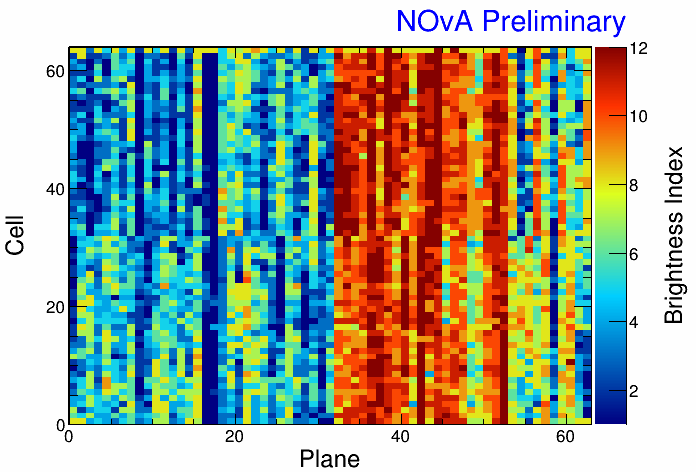
\includegraphics[width=\textwidth]{Plots/NOvAExperiment/BrightnessIndex.png}
\end{subfigure}
%\hfill
\begin{subfigure}[b]{0.495\textwidth}
\centering
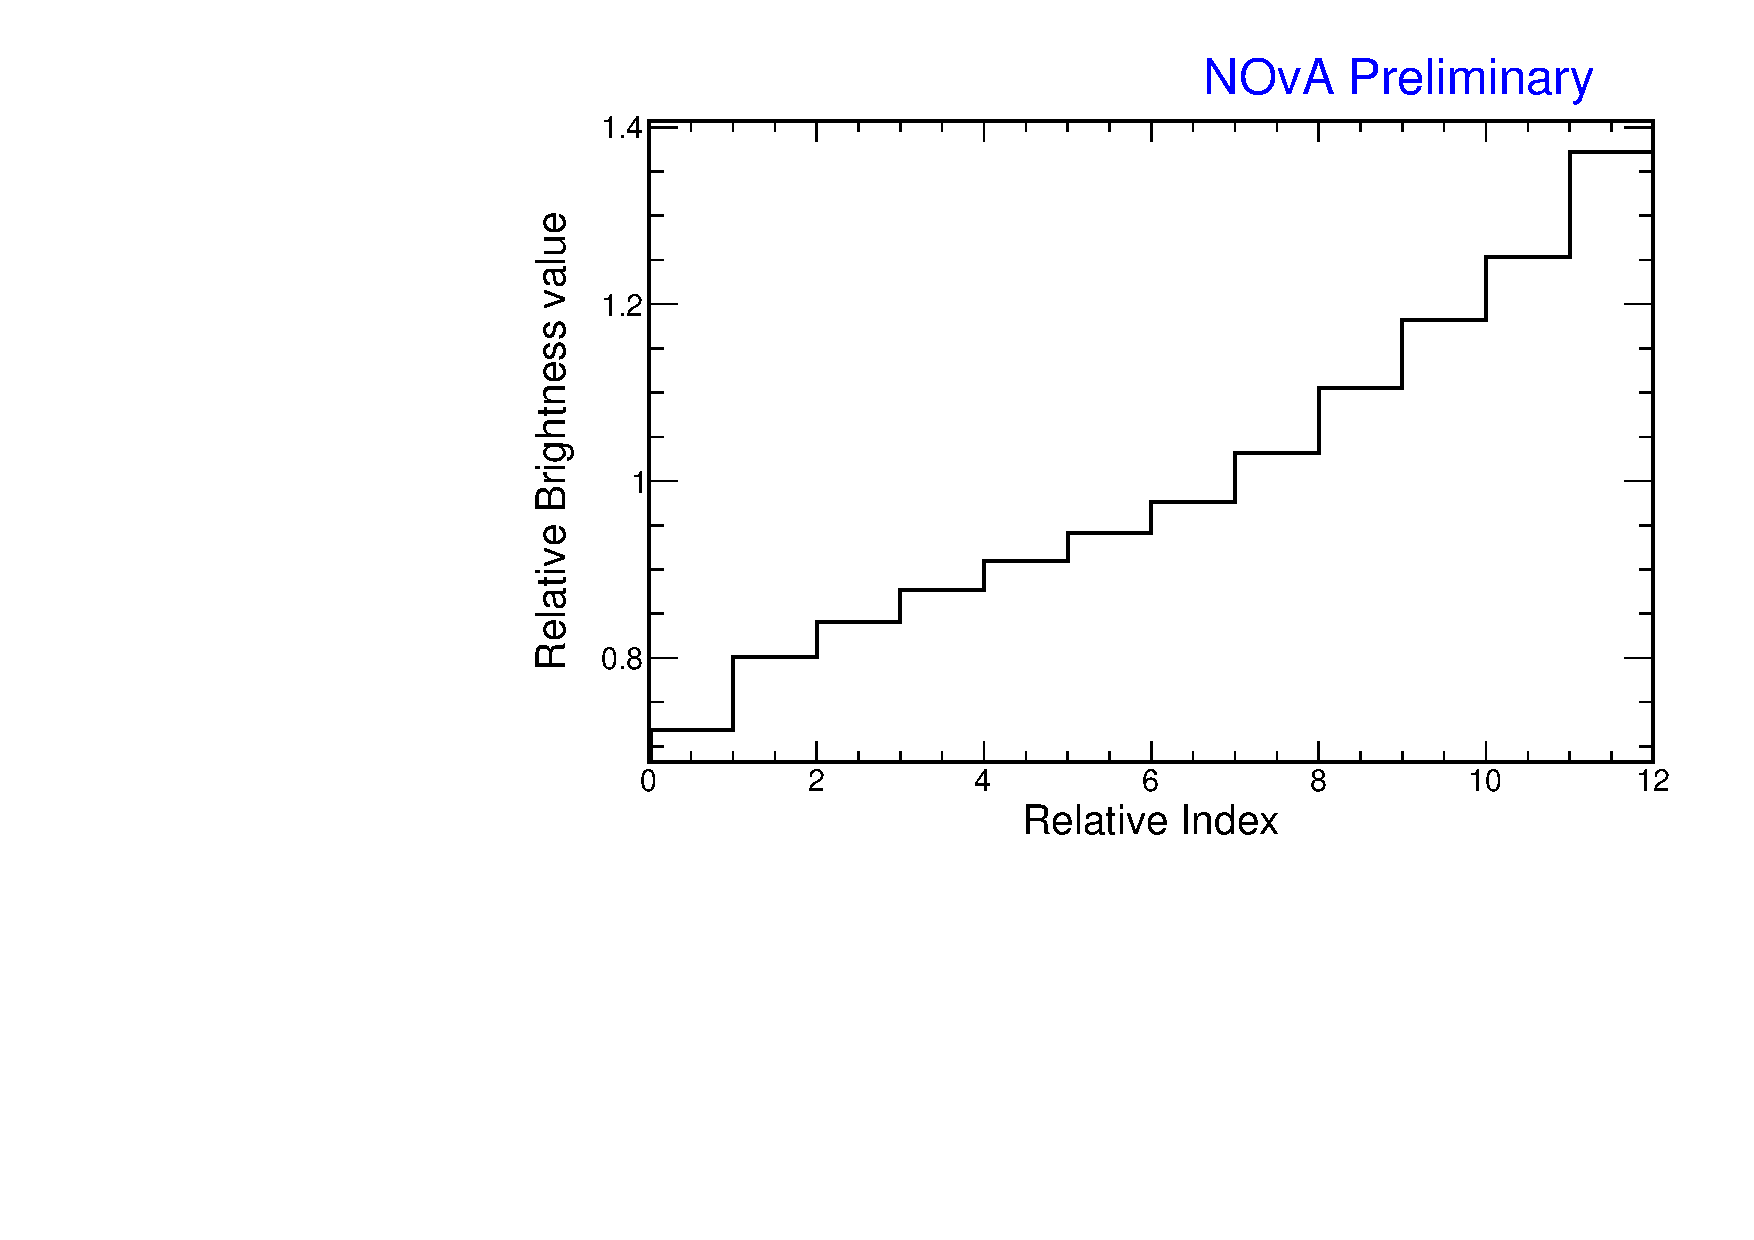
\includegraphics[width=\textwidth]{Plots/NOvAExperiment/BrightnessIndexToValue.pdf}
\end{subfigure}
\caption{The Test Beam detector is (like the standard NOvA detectors) divided into 12 brightness bins (left plot), each representing a relative difference in energy response (right plot) due to different brightnesses of the fibres, scintillators, or readout.}
\label{figFiberBrightnessBins}
\end{figure}

To divide each detector into the 12 brightness bins, we use results from the relative calibration. Specifically we take the result of the attenuation fit (equal to the average response) in the centre of each cell to fill a 2D histogram. Then we normalize this histogram by dividing the response in each $\textsf{Cell}\times\textsf{View}\times\textsf{Plane}$ by the average response in the corresponding $\textsf{Cell}\times\textsf{View}$. All uncalibrated cells get assigned the average response (1 in normalized histogram). Then we make a 1D histogram filled with the normalized responses of each cell and divide this histogram into 12 equally populated bins (so each bin represents approximately the same number of detector cells, shown on the left plot of Fig. \ref{figFiberBrightnessBins}). The mean normalized response in each bin represents the relative brightness value of this bin (right plot of Fig. \ref{figFiberBrightnessBins}).



%%% How do we divide the calibration. List the four parts (how about timing calibration? - talk about in DAQ)

\todo{Describe the absolute and relative calibration just in text}
The NOvA calibration consists of two parts \cite{NOVA-doc-7410}:
\begin{enumerate}
\item The \textbf{relative calibration} corrects for attenuation of scintillator light as it travels through the cell to the readout, as well as for differences between detector cells. This correction is calculated for each cell separately.
\item Followed by the \textbf{absolute calibration}, which only uses stopping muons when they are minimum ionising particles. In the absolute calibration we calculate a scale between the measured energy deposition, corrected by the relative calibration, and the simulated energy deposition in physical units of $\unit{MeV}$. This scale is calculated for each time period and each detector separately, which ensures the energy deposition is directly comparable wherever or whenever it occurred.
\end{enumerate}

%Calibration is necessary to convert electronic signals to physically meaningful energy in units of GeV. Two calibration steps precede the calorimetric energy calibration. First raw ADCs (Analogue Digital Conversion) are converted to units of photo-electrons (PE) using the known average response of the APDs; secondly an attenuation calibration corrects for the position dependent response [6]. A drift calibration may be included in the future to correct for changes in detector response over time. The calorimetric energy scale calibration is the last step in the calibration chain and the detector response should already be uniform in space and eventually also in time. [docdb:13579 - FA\_Calorimetric\_energy\_scale]

%Using the average expected APD response, integrated charge from the ADCs are converted to units of photo-electrons (PE) [SA Absolute energy scale]

%I think I should actually include some kind of a description of the ADC to PE conversion.
\iffalse
The scaling of the ADC to PE depends only on the gain and the version of the FEB. Otherwise it's just a very simple scaling (explain this at the PE definition):
\begin{equation}
PE=\frac{\textsf{peakADC}}{\textsf{ADCPerPE}},
\end{equation}
\begin{equation}
\textsf{ADCPerPE}=\textsf{Gain}\times\frac{4095}{ADCScale}
\end{equation}
where ADCScale is 217000 for FEBv4.1 and 204800 for FEBv5.2.
\fi

%The PECorr scaling is 75.0 (NDOS), 37.51 (ND), 39.91 (FD) and 39.91 (TB)

\todo{Just describe these units in text instead of here}
The basic units and variables used to define energy deposited in the NOvA detectors are listed in table \ref{tabCalibrationVars}.
\begin{table}[!ht]
\centering
\def\arraystretch{1.4}
\begin{tabular}{m{0.1\textwidth} m{0.84\textwidth}}
ADC & The digitized charge collected by the APDs from the \textbf{A}nalog to \textbf{D}igital \textbf{C}onverter \cite{NOVA-doc-13518}.\\
PE & Number of \textbf{P}hoto \textbf{E}lectrons. Calculated by a simple rescaling of the best estimate of the peak ADC. The PE per ADC scale only depends on the FEB type and the APD gain settings. This conversion is done before the calibration and PE serves as the base unit for calibration.\\
PECorr & \textbf{Corr}ected \textbf{PE} after applying the relative calibration results. The correction is a ratio between an average energy response (a pre-determined semi-arbitrary number) and the result of the the relative calibration fit (also called attenuation fit), which depends on w, cell, plane, epoch and detector. This makes the energy response equivalent across each detector.\\
MEU & \textbf{M}uon \textbf{E}nergy \textbf{U}nit is the mean detector response to a stopping cosmic minimum ionising muon.  For true variables it's equivalent to the mean MeV/cm and for reconstructed variables to the mean PECorr/cm.\\
MeV & Estimated energy deposited in the scintillator calculated from PECorr using the results of the absolute calibration. Additional correction for dead material needs to be made in order to get an estimate of the calorimetric energy.
\end{tabular}
\caption{Definitions of variables commonly used in calibration \cite{NOVA-doc-13579,NOVA-doc-7410}.}
\label{tabCalibrationVars}
\end{table}

\todo{Change this equation to be simpler and also include T/S corrections}
The final result of the NOvA calibration is the deposited energy in terms of physical units, which is in effect calculated as:
\begin{equation}
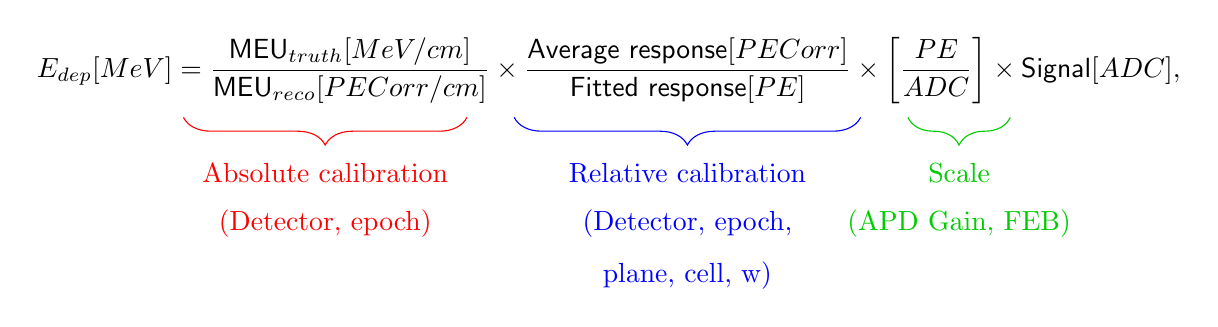
\begin{tikzpicture}[baseline=(current  bounding  box.center)]
\node {\(\displaystyle
E_{dep} [\unit{MeV}]=\frac{\textsf{MEU}_{truth} [\unit{MeV/cm}]}{\textsf{MEU}_{reco} [\unit{PECorr/cm}]}\times \frac{\textsf{Average response} [\unit{PECorr}]}{\textsf{Fitted response} [\unit{PE}]}\times \left[\frac{\unit{PE}}{\unit{ADC}}\right] \times \textsf{Signal} [\unit{ADC}],
\)};
\draw[decorate,decoration={brace,amplitude=10pt,mirror},red] (-5.4,-0.6) -- (-1.8,-0.6) node (A) [midway,yshift=-20pt]{Absolute calibration};
\node[below,yshift=-10pt,red] at (A) {(Detector, epoch)};
\draw[decorate,decoration={brace,amplitude=10pt,mirror},blue] (-1.2,-0.6) -- (3.2,-0.6) node (B) [midway,yshift=-20pt]{Relative calibration};
\node[below,yshift=-10pt,blue] (B2) at (B) {(Detector, epoch,};
\node[below,yshift=-10pt,blue] at (B2) {plane, cell, w)};
\draw[decorate,decoration={brace,amplitude=10pt,mirror},green!80!black] (3.8,-0.6) -- (5.1,-0.6) node (C) [midway,yshift=-20pt]{Scale};
\node[below,yshift=-10pt,green!80!black] at (C) {(APD Gain, FEB)};
\end{tikzpicture}
\end{equation}
where both the relative calibration results (blue fraction) and the absolute calibration results (red fraction) are stored in a database and applied together with the ADC-to-PE scale during processing of every hit in the NOvA detectors.

%The light is attenuated while traveling through the fiber. To find the correct energy of the incident particle these losses are corrected by using cosmic ray muons. The cosmic ray muons are used to calibrate the NOvA detectors because they provide a source of consistent energy across the detectors. The purpose of the attenuation calibration is to provide constants and formulae such that an amount of energy deposited in the detector and registered by an APD can be expressed in comparable units, PECorr which are the corrected photo-electrons (PE) no matter where the deposition occurred. Variations in time are to be handled by the drift calibration. The purpose of the absolute calibration is to provide a scaling factor, independent of channel since all of that variation should have been taken out by the relative calibration, so that energy deposits can be expressed in physically meaningful units (GeV).
%For both purposes cosmic rays are used as probes. For the attenuation calibration they represent a source of consistent energy deposits across the detector of approximately 1 minimum ionizing particle’s energy, MIP, but this is not assumed. Any average value consistent across the detector would do. For absolute calibration, stopping muons are used, whose precise energy deposits should be estimateable from the Bethe Bloch formula. [docdb:13579 - SA The Attenuation and Threshold Calibration of the NOvA detector, but a lot of this is actually just copied from Backhouse's original calibration technote docdb:7410]

%(Dividing data into periods and epochs) A new period is started for a major change to running conditions such as a horn current change, a long shutdown, target replacement, etc. Periods are divided into epochs. A new epoch is started whenever analysis or production reasons dictate. Calibration has been performed for all the periods separately and has used the data that are determined by the Data Quality group to be good. The effects of aging, temperature, partial filling, and cooling are neglected. The drift calibration should be able to account for all of these (but drift calibration doesn't really exist yet afaik). [docdb:13579 - SA The Attenuation and Threshold Calibration of the NOvA detector]


\subsection{Threshold and shielding correction}

Energy deposited far away from the readout may get attenuated enough to be shifted below the threshold. These low energy depositions would be missing from the attenuation fit, biasing it towards larger light levels with increasing distance from the readout. Similar effect, specifically for the vertical cells, is caused by using cosmic muons for calibration and applying it to beam muons. The top of the detector effectively shields the bottom, skewing the energy distribution of cosmic muons. To correct for both of these effect, we use the simulation pclist sample to calculate the threshold and shielding (also called threshold and shadowing) correction by comparing the true and reconstructed information. We apply this correction before the attenuation fits \cite{NOVA-doc-13579-SAAttenuationAndThreshold}.

%Should I write anything more? Maybe about how do we calculate this more specifically, or that it's done for view X fb bin X cell X w

%In the Far Detector data and MC a large divergence between calibrated and true energies as a function of W was observed [8]. This was traced back to the much longer cell lengths in the FD meaning that thresholds play a large role at the foot of a cell. Also self-shielding of the detector by its own mass lay a role in the observed discrepancy. Thresholds mean that for a hit to be seen by an APD, it may need to have a slight upwards fluctuation in the number of photons produced by the energy deposition. Self-shielding means that the average visible energy depositions from MIPs are not truly spatially uniform in the detector. If not corrected for these effects, there will be a bias in the set of hits that the attenuation fit sees, and leads it to overestimate the light-level, and so under-estimate real hit energies by tens of percent. The approach adopted to solve this problem was to create a correction factor as a function of view, cell, and position along the cell which would be applied before the attenuation correction to remove the effect of thresholds and shielding. To this end MC truth information about the calibration hit sample is used to create a combined threshold and shadowing correction for each cell and view combination,
%\begin{equation}
%T=\frac{PE}{\lambda}\frac{E_{true}}{E_{mip}},
%\end{equation}
%where $T$ is the combined “threshold and shielding” correction factor, $PE$ is the simulated photoelectrons recorded at the readout, $\lambda$ is the number of simulated photons which would be seen at the readout out in the absence of fluctuations, $E_{true}$ is the true energy deposited in the cell and $E_{mip}$ is the naive energy you would expect to be deposited based on the pathlength through the cell. In this way it encodes a threshold correction based on the simulated readout PE with and without the fluctuations, with $\lambda$ dependent on your simulated threshold, as well as a shielding correction based on the simulated energy deposition and a naive no shielding approximation. This equation gives us a cell by cell correction but we use an empirical polynomial fit to that distribution which removes statistical noise from the correction and well describes the initial distribution. This correction factor is applied to the cell by cell data and MC PE/cm distributions before the attenuation fits. [docdb:13579 - SA The Attenuation and Threshold Calibration of the NOvA detector, reference 8 is for docdb:7247, a talk by Backhouse]

\subsection{Relative calibration}\label{secRelativCalibration}

%Detailed description can be found in the "Instructions for the Attenuation Calibration Job" technote from Prabhjot from docdb:13579 (list of all calibration technotes) and on the relative calibration wiki page.

Relative calibration corrects for the attenuation of the scintillator light by fitting the average detector response over the position in each cell (w), separately for every cell inside each detector. Dividing the "average response" of the detector by the result of the attenuation fit for each $\textsf{Plane}\times\textsf{Cell}\times\textsf{w}$ combination effectively removes relative differences within and between all cells across the entire detector. The average response is a single constant number chosen to approximately represent the average response in the middle of the cell. Its value is for the far detector and Test Beam 39.91~PE/cm and for the near detector 37.51~PE/cm. The value of the average response has no impact of the calibration results, as the absolute scale of the detector response is determined during the absolute calibration and relative calibration only serves to remove the relative differences \cite{NOVA-doc-7410,NOVA-doc-13579-SAAttenuationAndThreshold}.
 
To create the attenuation fit we use the following procedure \cite{NOVA-doc-7410}:
\begin{enumerate}
\item Create the \textit{attenuation profiles}. Attenuation profiles are essentially profile histograms of detector response in terms of $\unit{PE/cm}$ as a function of position in the cell (w) for each cell in all planes. We construct the attenuation profiles over a little wider range than the actual length of the cell and always with 100 bins for each detector. This means that smaller detectors, like the Test Beam detector, have a finer binning ($\sim 3\unit{cm}$/bin) compared to the Far Detector ($\sim 18\unit{cm}$/bin).
\item Analyse the attenuation profiles. The job to create the attenuation profiles also creates validation histograms, which should be analysed prior to performing the attenuation fit to make sure the attenuation profiles look as expected.
\item Apply the threshold and shielding correction that was created before the relative calibration.
\item Do the attenuation fit over the full length of each cell. The fit consists of
\begin{enumerate}
\item an exponential fit, which combines two cases. First, when the scintillating light travels the short distance straight to the readout, and second, when it goes to the far side of the cell and loops around before going to the readout. The fitted function has a form:\\
\begin{equation}
y=C+A\left(\exp\left(\frac{w}{X}\right)+\exp\left(-\frac{L+w}{X}\right)\right),
\end{equation}
where $y$ is the fitted response, $L$ is the length of the cell and $C$, $A$ and $X$ are the fitted parameters. $X$ also represents the attenuation length.
\item Smoothing of the residuals from the exponential fit, mainly at the end of cells, with the LOcally WEighted Scatter plot Smoothing (LOWESS) method.
\end{enumerate}
\item Check the plots of the attenuation fit for a selection of cells.
\item Save the fit result to the database in the form of two csv tables. The \texttt{calib\_atten\_consts.csv} table holds the results of the exponential fit, together with the final $\chi^2$ of the fit. The \texttt{calib\_atten\_points.csv} table holds the results of the LOWESS smoothing.
\end{enumerate}

To ensure the quality of the attenuation fit, we only apply the results if the final $\chi^2<0.2$. If $\chi^2>0.2$, we ignore the results for this cell and mark it as \textit{uncalibrated}.

%Attenutation profiles have a constant binnin fNBins=100 (in w), same for ND, FD and TB. This results in an effectively finer binning for TB compared to ND and FD. For FD w = (-900,+900), ND: (-250,+250), TB: (-150,+150). TB: 3cm/bin, ND: 5cm/bin, FD: 18cm/bin. What effect could this have on the relative calibration results? Particularly on the calibration shape?

%where y is the response, L is the cell length, C, A and X are the free parameters in the fit. X gives the attenuation length as well. Initially, the fit is to the central part of the cell, which is different for each detector. In addition to the approximately quartic behavior at the ends of every channel there are in many channels fairly large residuals. They don’t appear to follow any consistent pattern. The leading hypothesis is that these are due to varying fiber position within the cell. Usually the fiber lies in the corners of the cell, but if it is somehow twisted so that it rises into the center of the cell, then it should collect more light, to an extent comparable to what is seen here. To remove such an irregular pattern, the residual from the analytic fit is simply fit with LOcally WEighted Scatter plot Smoothing, LOWESS. The LOWESS curve at each point is formed from the weighted mean of the deviations. The weighting function is the traditional tri-cube, (insert equation, likely not needed for this technote) [docdb:13579 - SA The Attenuation and Threshold Calibration of the NOvA detector, already in 1stAna and Backhouse's technote]

%For NDOS the fit was a very little bit different, where we didn't use $L$ but $3L/2$. Also it says that "Over the length of an NDOS cell, the effect of the long attenuation length is imperceptible, and is modelled as a constant (If you put a long attenuation term in, the fit drives the length scale to infinity anyway). [docdb:7410]

%In many channels, fairly large residuals are visible. They don’t appear to follow any consistent pattern. The hypothesis is that these are due to varying fibre position within the cell. Usually the fibre lies in the corners of the cell, but if it is somehow twisted so that it rises into the centre of the cell, then it should collect more light, to an extent comparable to what is seen here. To remove such an irregular pattern, the residual from the analytic fit is simply fit with LOWESS (locally weighted scatterplot smoothing). The LOWESS curve at each point is formed from the weighted mean of the deviations. The weighting function is the traditional tri-cube:
%\begin{equation}
%w_i=\left(1-\left|\frac{x-x_i}{\sigma}\right|^3\right)^3.
%\end{equation}
%The smoothing length scale $\sigma$ is 30cm. 20 points calculated by this method are stored, to be linearly interpolated between to approximate the full LOWESS curve. If the LOWESS fit at any point exceeds 15\% the original attenuation fit was very bad, and the channel is marked uncalibrated. Figure 4 shows an example of large (10\%) deviations being fitted. This variation is not seen in the MC, and so the LOWESS fit is skipped there. Due to the lower stats available in MC, instead of being collated by plane and cell, the curves are only calculated by view and cell. [docdb:7410]

%The current value of $\sigma$ in the code is $1.5\times\textsf{DetWidth}/20$

\subsection{Absolute calibration}

To find the absolute energy scale, we apply the relative calibration results on the stopping muon sample and look at the energy they deposited in cells 1-2 meters from the end of their tracks. In this track window they are approximately minimum ionising particles and their energy deposition is almost constant and well understood. Additionally, we don't use hits from the edges of a cell, as those might be affected by the lower number of events, fibre endings, or loops. 

For each calibrated data and simulation sample we take a mean of the corrected deposited energy distribution, separate for each view. We then take a simple average from the two views to get the final $\textsf{MEU}_{reco}$ in units of $\unit{PECorr/cm}$ for each sample \cite{NOVA-doc-13579-FACalorimetricEnergyScale}. Additionally, from simulation we can get the mean of the distribution of the true deposited energy in the scintillator, $\textsf{MEU}_{truth}$ in units of $\unit{MeV/cm}$ for the same sample of stopping muons. 

We ignore the energy that is lost in the dead material (PVC extrusions) and deal with it separately. The absolute energy scale for each sample is then the ratio of $\textsf{MEU}_{truth}/\textsf{MEU}_{reco}$. We save these absolute energy scales in another csv table called \texttt{calib\_abs\_consts.csv} which stores the $\textsf{MEU}$ values and their errors.

As part of the absolute calibration we also produce validation plots that show the effect of calibration on the distribution of the stopping muons. We analyse these plots and if everything looks all right we load all the csv tables into the database.

%Stopping muons provide a good sample of known energy deposits. If we can collect a “golden” sample, they should provide the scale factor to convert PECorr to GeV. So far, the method used has been imperfect, and the absolute calibration constants are known to be off by approx. 10\%. Since a factor already has to be derived to correct for dead material, this is not significantly impeding current efforts, but work was recently gone into improving this area. [docdb:7410 - this was likely before the track window cut was introduced] (Here it says that it's not such a big a problem since we have to scale for the dead material anyway. But nowadays we have to account for a large systematic uncertainty in the absolute energy scale in our analyses. How is the dead material correction different from the energy scale uncertainty?)

%...the calibration of the calorimetric energy scale of the NOvA detectors uses the energy deposited by stopping muons as a standard candle. To reduce systematic uncertainties, only those energy deposits in a 1-2 m window away from the muon track end point are used. The mean of the detector response distribution is found for data and MC in both near and far detectors. The mean of the distribution of true energy deposits in the track window is used to provide a conversion factor between the detector response and the true energy deposited in the scintillator for minimum ionising muons. The simulated dE/dx is uniform within about 1.8\% for hits around the minimum between 100-200 cm from the track end. The energy that a muon deposits within each cell is estimated using Geant 4 and stored in Fibre Liquid Scintillator (FLS) hits. FLS hits are only those within the active material (liquid scintillator) and energy loss within the passive material (plastic extrusions) is ignored. an estimate of the minimum energy loss rate of stopping muons in the NOvA scintillator is found to be,
%\begin{equation}
%\left.\frac{dE}{dx}\right|_{\textsf{mip}}=\left(1.7915\pm 0.0035\right)\unit{MeV/cm}.
%\end{equation}
%For stopping muons in NOvA it is also important to consider their decay. The muon has a vacuum lifetime of about 2.2 microseconds and favourably decays, with a branching ratio approx. 100\%, into an electron, an electron anti-neutrino and a muon neutrino. The electron produced in this decay is called a Michel electron and is used to select muons that stop within the NOvA detectors. The energy scale calibration is performed using cosmic ray muons. The calibration measures the detector response in data and MC in both near and far detectors and normalises them all by providing a conversion factor, for all four cases, that converts the detector response to energy in GeV. The energy loss rate (dE/dx) of stopping muons is well described by the Bethe-Bloch and is a function of the distance from the stopping point. A track window technique is used to minimise the variations in detector response that depend on the distance to the track end. Using this technique only hits within a region of distances from the track end are used. The position of the track window is chosen such that a mis-reconstruction of the track end point has the minimum effect on the mean detector response. The track window is currently set to be in the range from 100 cm to 200 cm from the track end.[docdb:13579 - FA\_Calorimetric\_energy\_scale]

%\FloatBarrier
%\newpage

\section{Systematic Uncertainties at NOvA}\label{sec:NOvASystematics}

\subsection{Systematic Uncertainties Related to the NOvA Neutrino Beam}

Hadron production and focusing systematic uncertainties

Principal component analysis

Maybe briefly also mention the POT scaling normalization uncertainty.

\subsection{Systematic uncertainties for NOvA detectors}

\subsubsection{Neutrino interaction systematic uncertainties}

\subsubsection{Energy scale systematic uncertainty}

%WORK IN PROGRESS

%First Analysis systematic uncertainties due to calibration:
%Sources of systematic uncertainty of particular concern are those introduced by residual variations remaining after calibration. Systematic errors are introduced by spatial and temporal variations in detector response. Further, any difference between the two detectors may introduce a relative shift in the energy scale between the detectors. A source of systematic uncertainty can be introduced by mis-reconstructing the end point of the muon track. Such a mis-reconstruction would shift the window within which hits are selected and hence the dE/dx of the muon.  The figure shows that the detector response varies by up to about 60\% over the range from 0 to 500 cm to the track end. This large variation illustrates the importance of careful consideration of the track window position and size. The detector response for both data and MC is minimum at about 130 cm from the track end and is flat to about 1\% in the range from 100 cm to 200 cm from the track end. For a track window starting at 100 cm from the track end, a conservative mis-reconstruction of the track end point by 10cm will shift the start of the track window to between 90cm and 110cm. This shift will alter the MEU value by less than 0.4\% over the range.
%If the calibration procedure was ideal the detector response would not vary with position in either data or MC. The calibration is not ideal and the detector response and recorded simulated energy deposition varies with position of the hit within the detector, such variations will introduce systematic errors. The position of a hit can be defined by the plane, cell within the plane, and distance along the cell (w) of the hit. The variation in detector response and simulated energy deposition vs. plane, cell and w for each view has been studied to quantify the systematic uncertainty introduced by these sources.
%The rise in detector response at the far end of FD y-view cells is an issue with several potential sources. The rise in response may be due to an acceptance effect or a light-level threshold effect among other possibilities. An acceptance effect is where greater energy must be deposited at the far end of the cells so that the light can travel along the fibre, hit the APD and be recorded as a hit. Both an acceptance effect and a light-level effect would introduce a bias towards higher energy hits toward the far end of cells.
%Another source of systematic uncertainty is introduced by the variation in detector response with time. The FD response is stable to about 1\% during the period from October 2014 to March 2015. The ND response needs further study but there was no significant trend over 6 months at 5\%. 
%As mentioned in Section 5, the version (7.1) of the calibration used for first analysis has been adjusted based on studies of muons from beam neutrinos interacting in the detector [8]. A shift of 3.6\% was introduced based on the average response of muons where large sections of the track were used. When only a track window of 100-200cm is used on the beam muons the difference is only 2.7\% [8]. Our best hypothesis for this residual 2.7\% difference is that it is caused by showery events that are present in ND data but not ND MC: it was shown in [9] that doing the calorimetric energy scale calibration using a truncated mean (or a median or a fit to the peak) gave a data/MC ratio that differed by 2.7\% compared to using the untruncated mean as described in this document. A comparison of various cross checks of the calorimetric energy scale was undertaken (in [10] and [11]) and concluded that the nearly 5\% difference between ND data and MC seen in a sample of Michele electrons [12] should be applied as both an absolute and relative shift to the calorimetric energy scale. The difference between the level of calorimetric energy resolution of stopping muons was studied and it was found that data and MC agreed best when an 8\% additional smearing was introduced. Studies for the NuMu analysis indicated that this was a negligible systematic uncertainty [13]. 
%[docdb:13579 - FA\_Calorimetric\_energy\_scale]

\subsubsection{Cell edge calibration systematic uncertainty}

\subsubsection{Detector ageing systematic uncertainty}

%Also include Chenerkov and light level tune uncertainties